\chapter{Rivelatori per neutroni lenti}
Si parla di neutroni lenti quando si ha a che fare con neutroni con un energia inferiore a 0.5 eV, detta anche \textit{cadmium cutoff}, in quanto
una reazione importante del cadmio si posiziona a quell'energia.
Quando si ha a che fare con i neutroni lenti spesso si eseguono operazioni di rivelazione piuttosto che di spettroscopia, in quanto le reazioni
che permettono di misurare direttamente l'energia del neutrone non hanno una sezione d'urto grande.
Vediamo le reazioni utilizzate.
\section{Reazioni nucleari con neutroni a bassa energia}
Le reazioni che vengono utilizzare nella rivelazione di neutroni sono a sezione d'urto elevata (almeno nel barn) in modo da avere rivelatori
di dimensioni ridotte.
Questo aspetto  \`e importante in quanto vengono utilizzati anche rivelatori a gas.
Sono, inoltre, utilizzati materiali ad elevata abbondanza isotopica o con arricchimento a basso costo, in modo da avere quantit\`a elevate di materiale
a basso costo.\\
Le reazioni che vengono utilizzate coinvolgono spesso fotoni che devo essere in grado di discriminare bene, in modo da distinguerli dal fondo e rivelare
in modo efficace i neutroni.
Sempre per questo scopo, vengono utilizzate quelle reazioni che hanno un Q-valore elevato ($Q=(m_i^{TOT}-m_f^{TOT})c^2$) in modo da avere fotoni ad energia
elevata e distinguerli pi\`u facilmente dal fondo (anche con semplici metodi basati sull'ampiezza); esse devono essere fortemente esotermiche
per svincolarci dall'energia del neutrone incidente (in quanto essa \`e bassa) e non avere energia di attivazione.
I prodotti di reazione sono spesso fotoni, particelle cariche pesanti, pezzi di fissione o altri neutroni, si cerca di utilizzare
quelle reazioni che producono particelle a range piccolo, in modo da avere dimensioni del rivelatore ridotte e misurare completamente l'energia
associata.\\
Se queste richieste sono rispettate, il risultato di una rivelazione di neutroni consiste in un picco posizionato al Q-valore della reazione
(fig.~\ref{fig:piccoNeutroni}).
\begin{figure}[htbp]
\begin{center}
	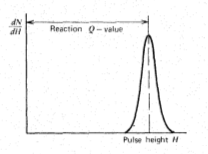
\includegraphics[scale=1]{./Immagini/PiccoNeutroni.png}
\caption{Picco dovuto alla rivelazione di neutroni lenti}
\label{fig:piccoNeutroni}
\end{center}
\end{figure}
\subsection{La cattura neutronica}
\`E la reazione di maggiore interesse, un neutrone lento, se passa sufficiente tempo vicino al nucleo, viene catturato formando un nuovo nucleo eccitato:
\begin{equation*}
\text{n} + ^A\text{X} \to ^{A+1}\text{X}^*
\end{equation*}
I tempi di vita dello stato eccitato possono essere variabili, se essi sono brevi il decadimento dar\`a luogo ad un nucleo diverso con emissione di particelle
$\alpha$ o protoni, altrimenti si parler\`a di stato metastabile e decader\`a nel ground state con emissione di fotoni.
La sezione d'urto di questo processo dipende fortemente dalla struttura interna del nucleo: esse possono andare da pochi millibarn a migliaia di barn,
la dipendenza della sezione d'urto \`e $\sigma_C \propto \frac{1}{v_n}$, per cui neutroni pi\`u lenti possono essere catturati pi\`u facilmente.\\
Una reazione molto importante \`e quella di formazione del deutone (ovvero il nucleo del deuterio):
\begin{equation*}
\text{n}+\text{p} \to \text{d} + \gamma
\end{equation*}
La sezione d'urto del processo risulta:
\begin{equation*}
\sigma_C = \frac{6.2 \cdot 10^4 \, \text{barn}}{v \, \text{(cm/s)}}
\end{equation*}
\subsection{La fissione}
In seguito alla cattura, un nucleo si scinde in due nuclei di massa comparabile pi\`u qualche neutrone.
La sezione d'urto per questo processo \`e di qualche centinaio di barn per neutroni termici.
\section{Reazioni importanti}
\subsection{Cattura del $^{10}$B}
La reazione \`e
\begin{equation*}
\text{n} + ^{10}\text{B} \to ^7\text{Li} + \alpha
\end{equation*}
Nel 94\% dei casi, il litio prodotto \`e nello stato eccitato e decade in $10^{-13}$ s nel g.s. con emissione di un fotone.
La reazione non dipende dall'energia del neutrone, quindi non pu\`o essere usata per effettuare spettroscopia.
L'energia dei due corpi \`e ben nota: poich\`e \`e noto il Q-valore e il neutrone \`e lento, si pu\`o approssimare tutto come un decadimento back-to-back
ed \`e possibile calcolare l'energia dei singoli corpi (nell'ordine del MeV).
La sezione d'urto del processo \`e circa di 4000 barn per n. termici, poi scala senza strutture con la velocit\`a.
\subsection{La cattura del $^{6}$Li}
\begin{equation*}
\text{n} + ^{6} \text{Li} \to ^3 \text{He} + \alpha
\end{equation*}
La sezione d'urto per n. termici \`e circa 1000 barn, poi scala come l'inverso della velocit\`a fino a 200 KeV dove c'\`e una risonanza.
\subsection{La cattura $^{3}$He}
\begin{equation*}
\text{n} + ^{6}\text{He} \to ^2\text{H} + \text{p}
\end{equation*}
La sezione d'urto \`e circa 5000 barn, poi scala, il rivelatore \`e costoso in quanto $^3$He non \`e molto abbondante, il Q-valore \`e circa 800 keV.
\subsection{Cattura radiativa del $^{157}$Gd}
Il gadolinio \`e un materiale ad altissima sezione d'urto di cattura ($\approx 255000$ barn), questo permette di poter costruire
rivelatori di neutroni molto sottili mantenendo una buona efficienza di rivelazione.
In seguito alla cattura il gadolinio emette fotoni o elettroni di conversione, l'elettrone pi\`u emesso \`e a 72 keV con un branching ratio del 39\%.
Questo elettrone pu\`o essere utilizzato per localizzare l'interazione, utilizzando ad esempio un film fotografico che registri la posizione di interazione.\\
Un'altra tecnica prevede l'uso di scintillatori con una piccola frazione (0.5\%) di Gd per rivelare i neutroni, il problema di questa tecnica sta nel
distinguere l'evento dal fondo.
\section{Rivelatori basati sul boro-10}
\subsection{Tubo proporzionale a BF$_3$}
Un rivelatore possibile \`e basato sulla camera proporzionale riempita con BF$_3$, dove si utilizza boro-10;
il gas opera ad una pressione di 0.5-1 atm e l'abbondanza del boro pu\`o essere portata al 100\% ottenendo ottime efficienze.
Lo spettro atteso dal rivelatore risulta quindi formato da due picchi (fig.~\ref{fig:spettroAttesoBF3}) dovuti ai due possibili decadimenti del boro,
inoltre ci si aspetta che le aree siano in un rapporto di 93:6.
\begin{figure}[htbp]
\begin{center}
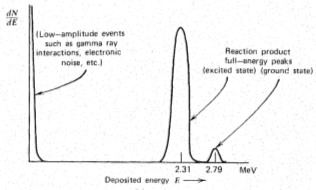
\includegraphics[scale=1]{./Immagini/SpettroAttesoBF3.png}
\caption{Spettro atteso in un tubo BF$_3$}
\label{fig:spettroAttesoBF3}
\end{center}
\end{figure}
Sperimentalmente viene osservato uno spettro come in fig.~\ref{fig:spettroSperimentaleBF3}.
\begin{figure}[htbp]
\begin{center}
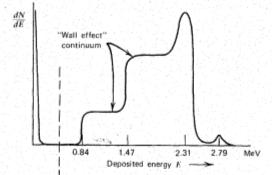
\includegraphics[scale=1]{./Immagini/SpettroSperimentaleBF3.png}
\caption{Spettro osservato sperimentalmente in un rivelatore BF$_3$}
\label{fig:spettroSperimentaleBF3}
\end{center}
\end{figure}
Il motivo di questo spettro \`e dovuto al fatto che posso avere fughe di radiazione che non vengono misurate (effetto parete), dando luogo
al continuo; in particolare posso avere una fuga di sola $\alpha$ o una fuga di solo litio, ma non di entrambi, in quanto essendo emessi
back-to-back, se una particella viene prodotta vicina alla parete ed esce, l'altra andando in verso opposto verr\`a completamente misurata.\\
I rivelatori sono costruiti con anodi di dimensioni delle decine di $\mu$m e tensioni operative di 2-3 kV;
l'anodo pu\`o essere problematico per la sua capacit\`a di catturare neutroni, per questo vengono utilizzati anodi in alluminio, in quanto hanno
sezioni d'urto piccole.
Un problema in questi rivelatori \`e dato dagli impulsi spuri, essi possono essere generati da shock meccanici o fluttuazioni della corrente di fuga; inoltre hanno il problema dell'invecchiamento legato alla deposizione su anodo e catodo di residui da dissociazione molecolare.\\
Spesso ai neutroni sono associati dei fotoni, la loro discriminazione \`e facile a bassi rate, in quanto essi producono elettroni che liberano poca energia nei gas.
Questo diventa un problema ad alti rate, in quanto effetti di pile-up aumentano l'energia apparente e rendono pi\`u difficile la discriminazione;
l'invecchiamento pu\`o rendere difficile la discriminazione, per questo a volte si procede con una purificazione del tubo, per renderlo pi\`u resistente.\\
Per quanto riguarda l'efficienza, supponendo che il flusso incida contro il tubo in modo assiale, l'efficienza risulta:
\begin{equation*}
\epsilon(E) = 1 - e^{-\Sigma_a(E)\,L}
\end{equation*}
dove $\Sigma_a(E)$ \`e la sezione d'urto macroscopica ad energia E.
Valori tipici sono del 90\% per neutroni termici e del 3.8\% per neutroni a 100 eV.
\subsection{Rivelatori rivestiti con boro}
\`E possibile utilizzare una tradizionale camera proporzionale e successivamente rivestirne le pareti interne con boro per aggiungere la capacit\`a di
rivelazione dei neutroni; con questa tecnica si ottengono rivelatori pi\`u resistenti (il BF$_3$ non \`e il gas ideale per una camera proporzionale) ad alti rate di fotoni.
Il problema di questi rivelatori sta nello spettro: poich\`e i prodotti di reazione sono back-to-back, una delle due particelle non verr\`a rivelata
mentre l'energia della seconda verr\`a misurata in base all'energia che essa ha depositato nello strato morto di boro.
\begin{figure}[htbp]
\begin{center}
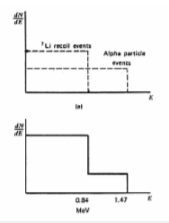
\includegraphics[scale=1]{./Immagini/SpettroRivestimentoBoro.png}
\caption{Spettro in un rivelatore con rivestimento al boro.}
\end{center}
\end{figure}
Poich\`e l'energia media depositata \`e inferiore, la discriminazione dei fotoni \`e pi\`u difficile.
\subsection{Scintillatori caricati con boro}
Nei tubi proporzionali c'\`e un grosso spread nel risetime rendendoli inutilizzabili per applicazioni T.O.F., un'alternativa sta nell'utilizzo di
scintillatori sottili caricati con boro.
Il problema di questi dispositivi sta nella difficolta di discriminare il fondo $\gamma$, gli elettroni secondari, infatti, depositano tutta la loro energia
e, inoltre, gli scintillatori organici rispondono con meno luce alle particelle pesanti cariche.
\section{Altri tipi di rivelatori}
\subsection{Rivelatori al litio}
Uno scintillatore tipico \`e il LiI, simile al NaI, la luminosit\`a \`e del 35\% rispetto allo scintillatore al sodio.
I tempi tipici di produzione della luce sono nei 300 ns e per spessori nell'ordine del cm l'efficienza \`e quasi pari a 1, per neutroni lenti.
Lo spettro prodotto \`e un picco di energia piena a 4.78 MeV, corrispondente ad un picco prodotto da elettroni a 4.1 MeV.
Essendo il rendimento in luce da particelle cariche pesanti simile a quello dovuto ad elettroni, la discriminazione del fondo gamma \`e difficile in questi dispositivi;
inoltre essi sono igroscopici.
\subsection{Contatori proporzionali ad elio-3}
I prodotti del decadimento dell'elio-3 hanno un Q-valore non molto grande e un range grande, per questo ci sono problemi legati all'effetto parete che
rendono difficile la discriminazione dai $\gamma$.
Questi dispositivi hanno un counting plateau stretto e una pressione di esercizio maggiore del bar, rendendoli pi\`u efficienti dei rivelatori BF$_3$. 